% !TeX root = ../dokumentation.tex

\chapter{Sprints}

\section{Sprint 1}
\todo{Beschreibung des Produktincrements}

\section{Ziele Sprint 1}
\todo{Ziel Sprint 1}

\section{Ergebnisse Sprint 1}

\subsection{Produktincrement}
\subsection{Charts}

\subsection{Probleme und Verbesserungen}
\todo{Retro Ergebnisse}


\subsection{Bearbeitete User Storys}

\subsubsection{Ticket 1}

\subsubsection{Ticket 2}

\section{Sprint 2}
\subsection{Produktincrement}
\subsection{Charts}
\subsection{Probleme und Verbesserungen}


\subsection{Bearbeitete User Storys}

\subsubsection{SKIOS-69 Preliminary ORM}
Das Ticket \enquote{SKIOS-69 Preliminary ORM} hatte folgende User Story:
\begin{quotation}
    Als Programmierer will ich eine Datendefinition in einer Datenbank
    haben, und diese als Packet einbinden können.
\end{quotation}
Diese wurde folgendermaßen gelöst:
\begin{quotation}
Die Datendefinition wurde durch TypeORM~\parencite{web/TypeORM} dargestellt.
Diese wurde in dem Repository skiosa/orm~\parencite{git/skiosa/orm} als NPM-Package~\parencite{web/npm} abgebildet.
Es wurden die Article von RSS-Feeds in dem Schema aus Abbildung~\ref{fig:databaseORM} abgebildet.
\begin{figure}
    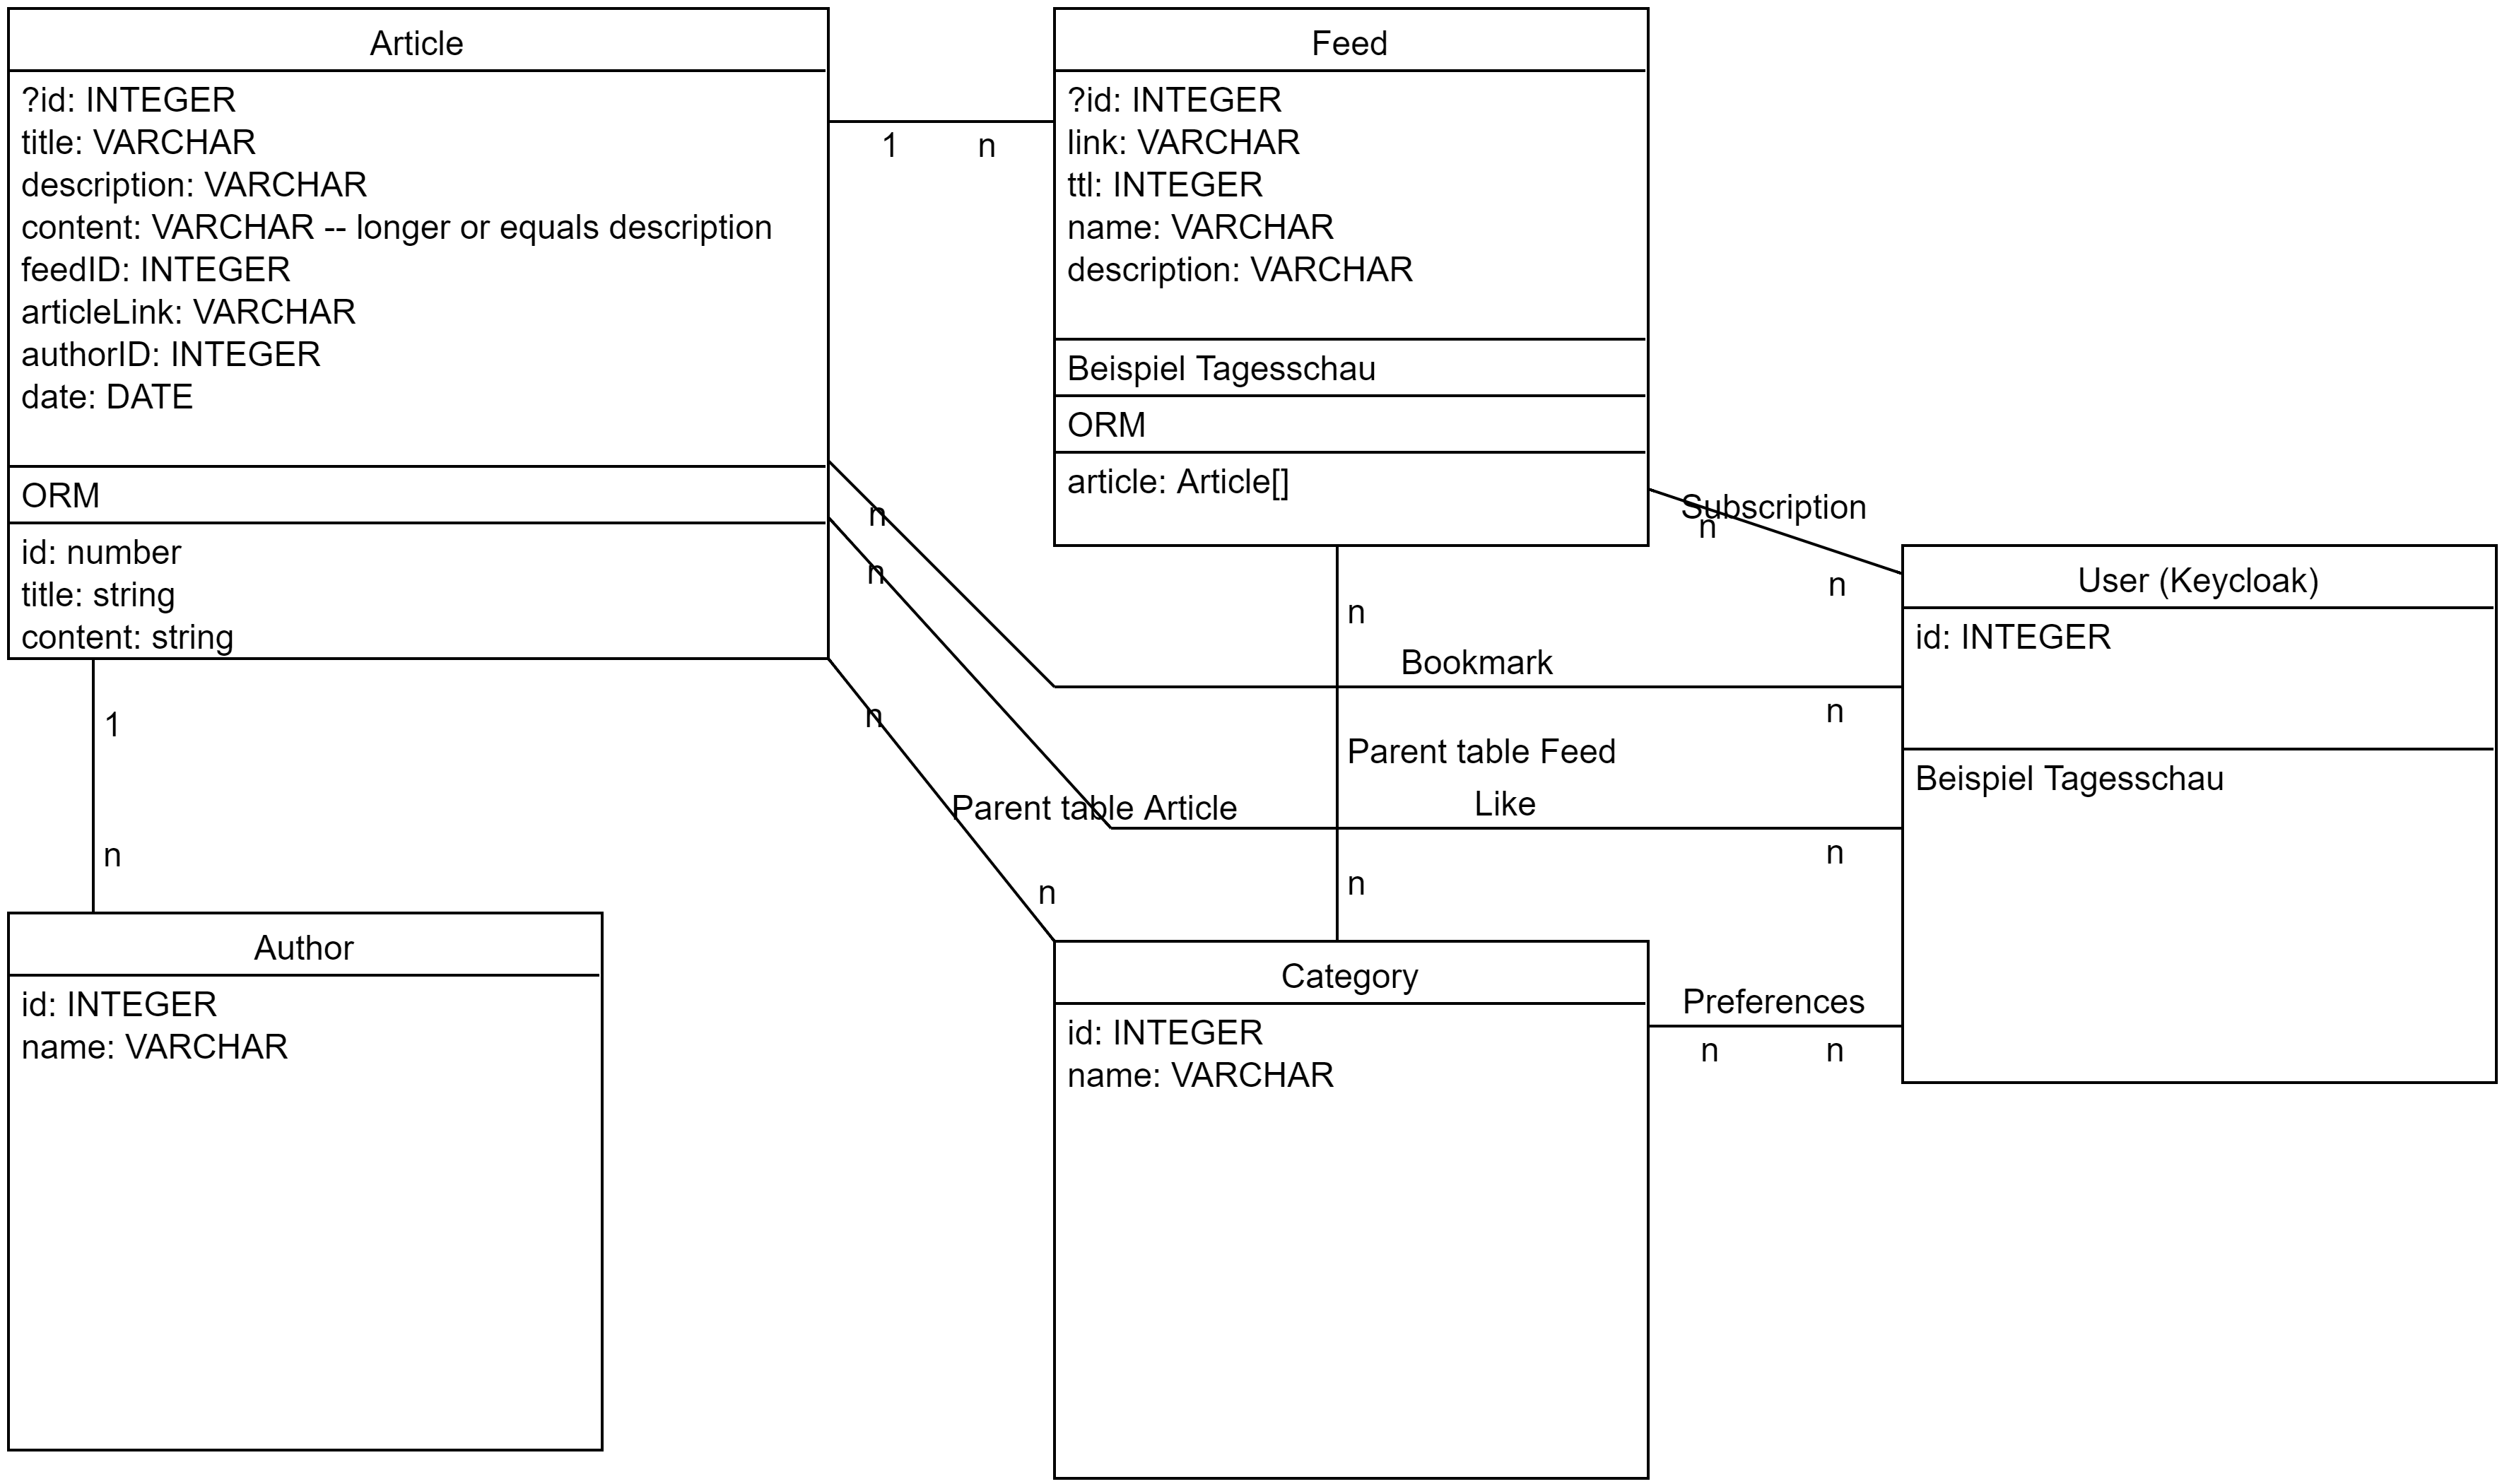
\includegraphics[width=\linewidth]{Database_Model.png}
    \caption{Datendefinition innerhalb der Datenbank}
    \label{fig:databaseORM}
\end{figure}
\end{quotation}
Bearbeitet von Jonas Eppard und Tim Horlacher.

\section{Sprint 3}

\subsection{Produktincrement}
\subsection{Charts}
\subsection{Probleme und Verbesserungen}


\subsection{Bearbeitete User Storys}
\subsubsection{SKIOS-116 Structure and table of contents for submission (\LaTeX)}
Das Ticket \enquote{SKIOS-116 Structure and table of contents for submission (\LaTeX)}
hatte folgende User Story:
\begin{quotation}
    As a team member, I would like to have a rough structure to orient myself while writing our submission documentation.\\
    For this story, please read the requirements and guidelines set out by Garidis and develop a rough idea on how to structure our \LaTeX project.\\
    \textbf{Acceptance Criteria}
    \begin{itemize}
        \item Table of contents is created (with \textbackslash{}section, \textbackslash{}subsection, etc.) in \LaTeX
        \item Structure reflects guidelines of Garidis
        \item Structure is explained in confluence page
        \item Existing \LaTeX~stories have a defined place where their pages will go
    \end{itemize}
\end{quotation}
Dies wurde folgendermaßen gelöst:
\begin{quotation}
    Es wurde die Struktur dieses \LaTeX-Dokuments angelegt. Hierbei musste nur das Inhaltsverzeichnis
    angelegt werden, da das \LaTeX-Template schon vorhanden war.
    Die Verwendung wurde in Confluence dokumentiert.
\end{quotation}
Bearbeitet von Jonas Eppard.
